\documentclass[journal,onecolumn]{IEEEtran}
\ifCLASSINFOpdf
  \usepackage[pdftex]{graphicx}
  \DeclareGraphicsExtensions{.jpg}
\fi

\usepackage{subcaption}
\usepackage{hyperref}

\begin{document}
\title{Homework 2 Report – Computer Vision \& Deep Learning}

\author{Lev~Chelyadinov,~\IEEEmembership{B18-SE-01 Student,~Innopolis~University}}% <-this % stops a space

\markboth{Innopolis University, December 2021}%
{Chelyadinov: Homework 2 Report}

\maketitle

\section{Introduction}

\IEEEPARstart{T}{his} report describes the process of training state-of-the-art object detection models on a custom dataset, created, annotated and loaded manually. Three models were covered – \emph{YOLOv4 Tiny}, \emph{YOLOv5 Nano}, and \emph{Mask R-CNN}. The task at hand is to detect taps in photos and determine whether the water is running in them or not. This could allow for no-hardware detection of water that has been left running to avoid floods and over-consumption.


\section{Dataset}

\subsection{Creation of images}

The dataset for training models to this task was captured with a 16 megapixels smartphone camera. Every tap was captured three times in both states. This was done to enable the model to learn what a tap looks like from different angles.

The taps were chosen in public places of Innopolis, however, a few of them are from private dormitory rooms, photographed with permission from inhabitants.

\begin{figure}[htb]
    \centering
    \begin{subfigure}[b]{\textwidth}
        \centering
        \includegraphics[width=0.475\linewidth]{figures/sample-run-1.jpg}%
        \hfill
        \includegraphics[width=0.475\linewidth]{figures/sample-no-run-1.jpg}
    \end{subfigure}
    \caption{Samples from the original dataset}
\end{figure}

\subsection{Annotation}

In order to make the dataset compatible with all three target models (\emph{YOLOv4}, \emph{YOLOv5}, \emph{Mask R-CNN}), the annotation had to be done around the object with a precise curve to create a mask over the image where the tap is. For this purpose, an online service, Supervisely\footnote{\href{https://supervise.ly/}{https://supervise.ly/}}, with a free \emph{Commnuity} plan was used. It provided an interface to create a mask and then export the resulting dataset.

\begin{figure}
    \centering
    \includegraphics[width=0.475\linewidth]{figures/sample-with-mask.jpg}
    \caption{Original image and the added mask of object annotation from Supervisely}
\end{figure}

Supervisely provides an option to export the PNG masks along with the images, but in practice it was not needed because the size of the exported dataset grew considerably and all of the necessary information was already available in the JSON annotations. The complete dataset, downloaded with the option ".json + images" is available in the \emph{Releases}\footnote{\href{https://github.com/illright/cvdl-save-water-iu-f21/releases}{https://github.com/illright/cvdl-save-water-iu-f21/releases}} section of the GitHub repository of this project, titled \texttt{original-dataset.zip}.

\subsection{Conversion for models}

Each model has its own format of data, therefore, in order to use the exported dataset from Supervisely, it first had to be converted to each model's specific data format

\subsubsection{YOLOv4}

The Darknet implementation\footnote{\href{https://github.com/AlexeyAB/darknet}{\texttt{AlexeyAB/darknet} on GitHub}} of YOLOv4 was chosen to represent the YOLOv4 architecture. The dataset was converted from Supervisely format to Darknet YOLO format with the help of another online tool, Roboflow\footnote{\href{https://roboflow.com/}{https://roboflow.com/}}, with its free \emph{Public} plan. It allows uploading images and annotations in a variety of formats and is capable of outputting a dataset that is suitable for Darknet. Moreover, Roboflow provides Python bindings that made it possible to deliver the dataset directly to the training code, without manually downloading and uploading the dataset.

In order to match the Darknet YOLOv4 format exactly, the data was resized to 416x416 pixels without preserving the aspect ratio. It affected the image, but not significantly, see \textbf{Fig. 3} for an example. Before that, Roboflow's suggested \emph{Auto-Orient} step was also applied, but it was not necessary as all of the images were oriented correctly from the start.

\begin{figure}
    \centering
    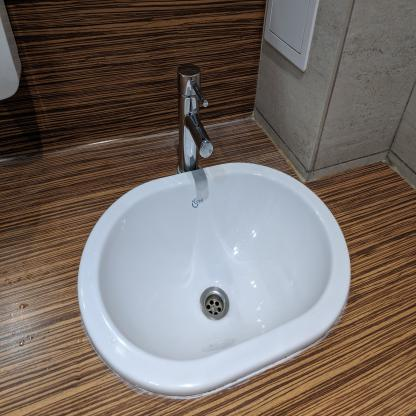
\includegraphics[width=0.475\linewidth]{figures/sample-416.jpg}
    \caption{A sample from the dataset after resizing to 416x416 pixels}
\end{figure}

\subsubsection{YOLOv5}

Similarly to YOLOv4, Roboflow provides an option to export the dataset in the format that is suitable for YOLOv5. The preferred image size of YOLOv5 is 640x640 pixels, so for training this architecture, the dataset was exported with an appropriate resizing step. Everything else remained the same as in the case of YOLOv4. The Ultralytics' implementation\footnote{\href{https://github.com/ultralytics/yolov5}{\texttt{ultralytics/yolov5} on GitHub}} of YOLOv5 integrated seamlessly with Roboflow.

\subsubsection{Mask R-CNN}

Matterport's implementation\footnote{\href{https://github.com/matterport/Mask_RCNN}{\texttt{matterport/Mask\_RCNN} on GitHub}} of Mask R-CNN does not define a particular data format, unlike the previous models. Instead, it suggests its users to implement a \texttt{Dataset} subclass in Python that would override the methods responsible for loading the dataset and the masks for images. This was done manually, the code of the dataset is provided in the Jupyter notebook file\footnote{\href{https://github.com/illright/cvdl-save-water-iu-f21/blob/main/notebooks/mask-rcnn.ipynb}{\texttt{notebooks/mask-rcnn.ipynb} in \texttt{illright/cvdl-save-water-iu-f21} on GitHub}} for training Mask R-CNN in the GitHub repository of the project.

Even though Mask R-CNN does not define an input format, the input images were still resized to 448x448 pixels without preserving aspect ratio, both to speed up training and to simplify the configuration.

\section{Training}

The training of the three architectures on the dataset of taps was carried out in Google Colaboratory\footnote{\href{https://colab.research.google.com/}{https://colab.research.google.com/}} to ensure GPU-accelerated computations. During the training, the free plan of Colaboratory was used, which yielded access to an NVIDIA Tesla K80 GPU.

Each model was trained in a separate Jupyter notebook. The notebooks with saved outputs may be found in the \emph{Releases} section of the GitHub repository for this project, while the source-only version of the notebook is checked into version control.

\subsection{YOLOv4}

As mentioned previously, for this task, the Darknet implementation of YOLOv4 Tiny was considered. The training notebook was built by close modeling of Roboflow's tutorial\footnote{\href{https://blog.roboflow.com/training-yolov4-on-a-custom-dataset/}{https://blog.roboflow.com/training-yolov4-on-a-custom-dataset/}} on training YOLOv4 on a custom dataset.

The notebook is titled \texttt{yolov4-tiny.ipynb}.

\subsection{YOLOv5}

YOLOv5 Nano was chosen to represent the YOLOv5 family of models as the smallest and fastest edition. The training notebook was again built according to Roboflow's tutorial\footnote{\href{https://blog.roboflow.com/how-to-train-yolov5-on-a-custom-dataset/}{https://blog.roboflow.com/how-to-train-yolov5-on-a-custom-dataset/}} on training YOLOv5 on a custom dataset. The tutorial covers YOLOv5 Small but the adaptation to Nano was trivial.

The notebook is titled \texttt{yolov5-nano.ipynb}.

\subsection{Mask R-CNN}

Mask R-CNN has no editions varying in size, unlike YOLOv4 and YOLOv5, so it was trained as is. The training notebook was adapted from the sample notebook (\texttt{samples/shapes/train\_shapes.ipynb}) in the Matterport's Mask R-CNN repository in accordance to the introductory blog post\footnote{\href{https://engineering.matterport.com/splash-of-color-instance-segmentation-with-mask-r-cnn-and-tensorflow-7c761e238b46}{https://engineering.matterport.com/splash-of-color-instance-segmentation-with-mask-r-cnn-and-tensorflow-7c761e238b46}} by Matterport.

The notebook is titled \texttt{mask-rcnn.ipynb}.

\section{Evaluation}

One of the main metrics to assess object detection models is \emph{mean average precision} (mAP). We will primarily focus on this metric when assessing the performance of the three models.

\subsection{Performance of YOLOv4 Tiny}

The Darknet implementation of YOLOv4 produces a chart during its training (see \textbf{Fig. 4}). It shows that mAP has reached 100\%, which could indicate that the model has trained to perform flawlessly, however, that is not exactly the case according to the inference on actual images on the test set.

\begin{figure}
    \centering
    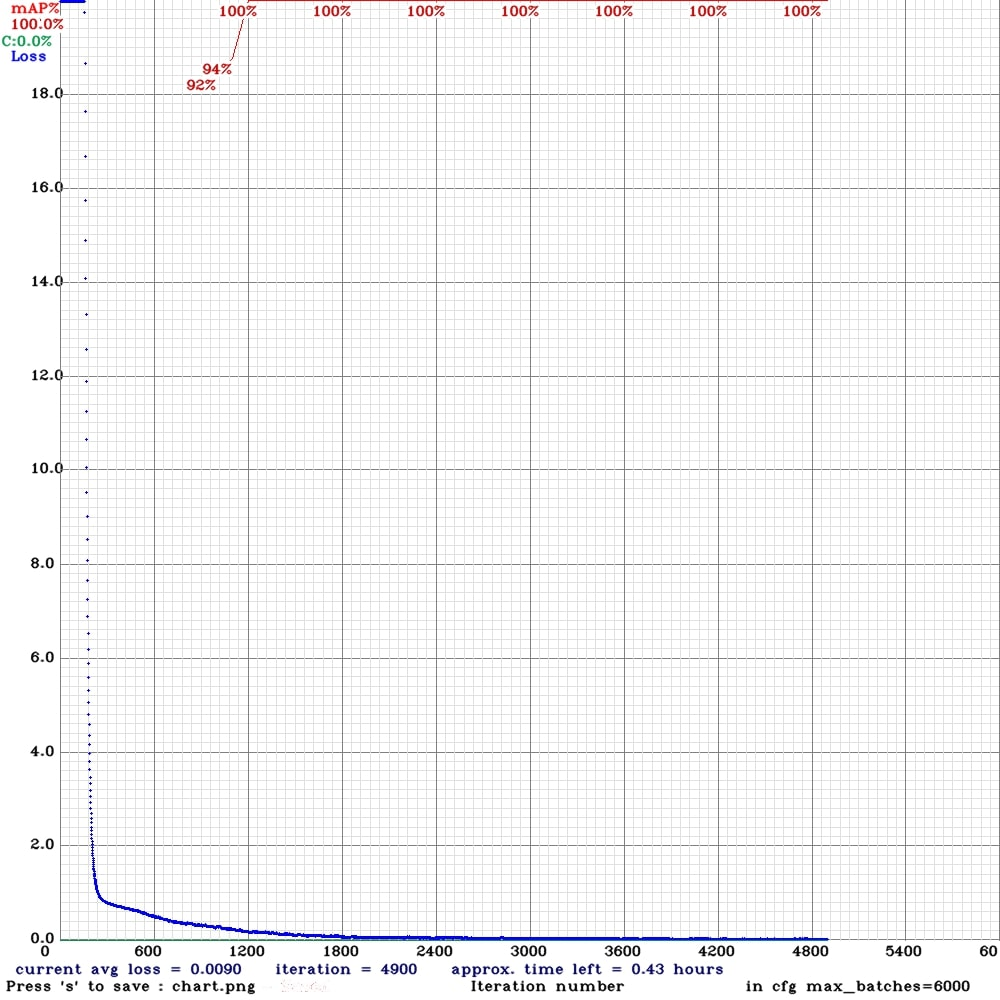
\includegraphics[width=0.475\linewidth]{figures/chart-yolov4.jpg}
    \caption{Loss and mAP during training of YOLOv4 Tiny}
\end{figure}

\begin{figure}[htb]
    \centering
    \begin{subfigure}[b]{\textwidth}
        \centering
        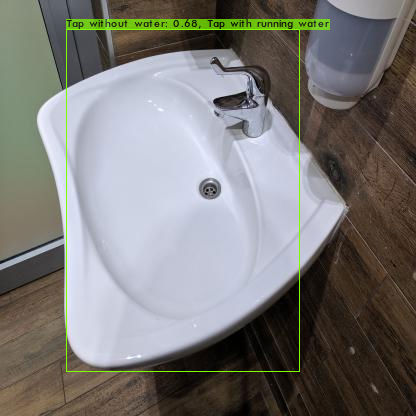
\includegraphics[width=0.475\linewidth]{figures/yolov4-prediction-1.jpg}%
        \hfill
        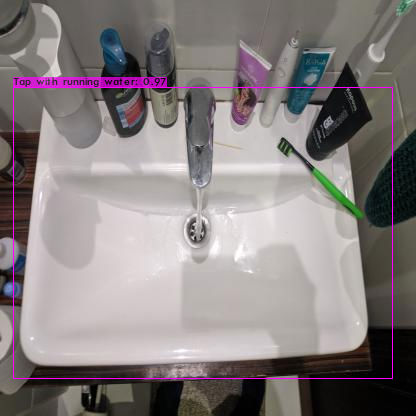
\includegraphics[width=0.475\linewidth]{figures/yolov4-prediction-2.jpg}%
        \hfill
        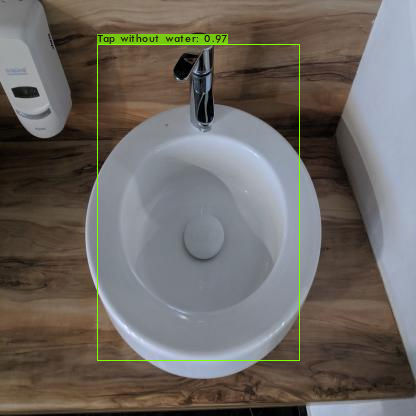
\includegraphics[width=0.475\linewidth]{figures/yolov4-prediction-3.jpg}%
        \hfill
        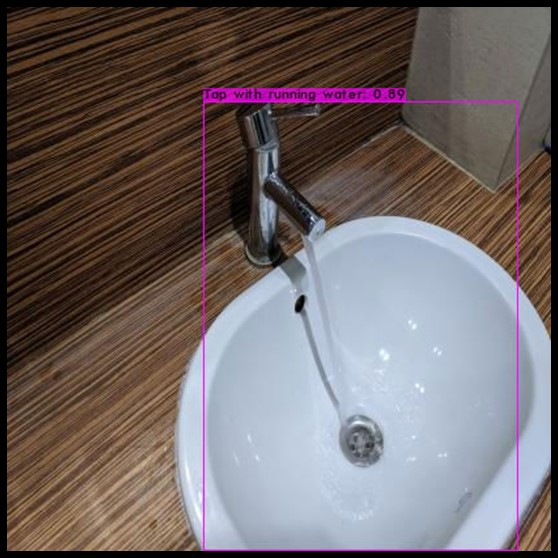
\includegraphics[width=0.475\linewidth]{figures/yolov4-prediction-4.jpg}%
        \hfill
    \end{subfigure}
    \caption{Predictions of YOLOv4 Tiny on the test portion of the dataset}
\end{figure}

As shown in \textbf{Fig. 5}, the model does not predict bounding boxes precisely. Additionally, sometimes, overlapping classifications occur. However, most of the time, the model predicts the correct class with sufficient amount of confidence and no false positives. As will soon become evident, these results are among the good ones for quite a challenging differentiation task.

\subsection{Performance of YOLOv5 Nano}

Ultralytics's implementation of YOLOv5 is integrated with Tensorboard, which provides insights to how mAP and average mAP across Intersection-over-Union (IoU) thresholds from 0.5 to 0.95 have changed throughout the training process. This implementation is also equipped with early stopping with a patience setting of 100 epochs, which means that the best results were obtained 100 epochs before the end. \textbf{Fig. 6} presents the charts of the aforementioned metrics and \textbf{Fig. 7} highlights that the model is unable to reliably make confident predictions. The inference was performed with a confidence threshold of 0.6, and many predictions weren't selected.

\begin{figure}[h]
    \centering
    \begin{subfigure}[b]{\textwidth}
        \centering
        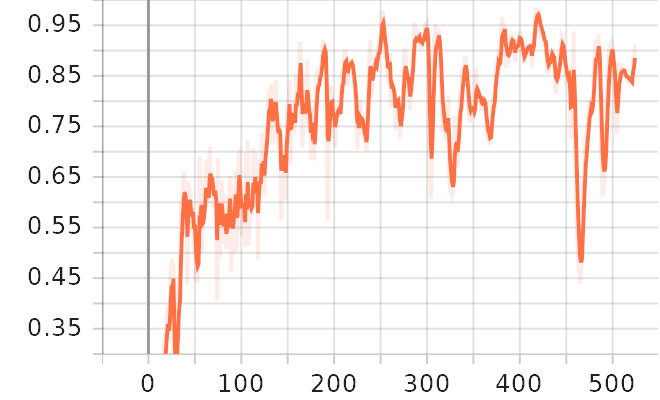
\includegraphics[width=0.475\linewidth]{figures/yolov5-map-chart.jpg}%
        \caption{mAP with IoU threshold of 0.5}
    \end{subfigure}
    \vfill
    \begin{subfigure}[b]{\textwidth}
        \centering
        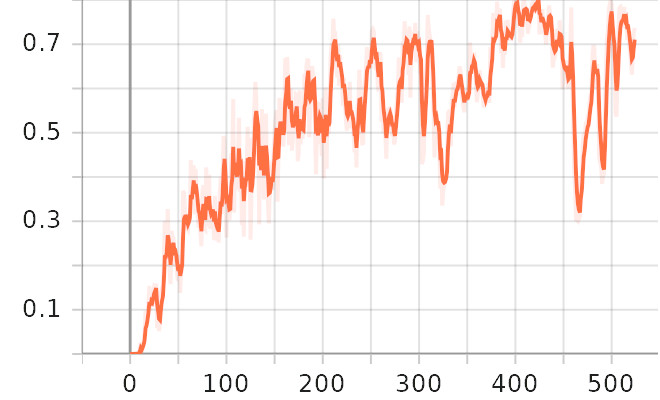
\includegraphics[width=0.475\linewidth]{figures/yolov5-map-95-chart.jpg}
        \caption{Average mAP with IoU thresholds from 0.5 to 0.95}
    \end{subfigure}
    \caption{Tensorboard charts of YOLOv5 Nano's performance during training. The horizontal axis counts the epochs of training.}
\end{figure}

\begin{figure}[htb]
    \centering
    \begin{subfigure}[b]{\textwidth}
        \centering
        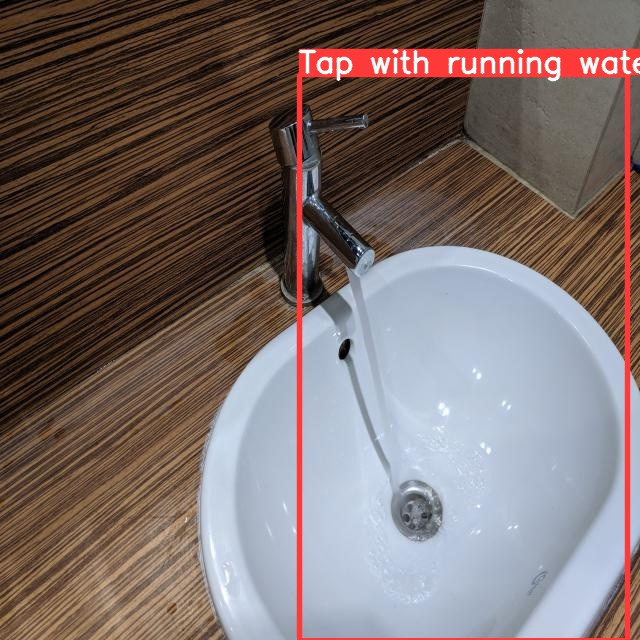
\includegraphics[width=0.475\linewidth]{figures/yolov5-prediction-1.jpg}%
        \hfill
        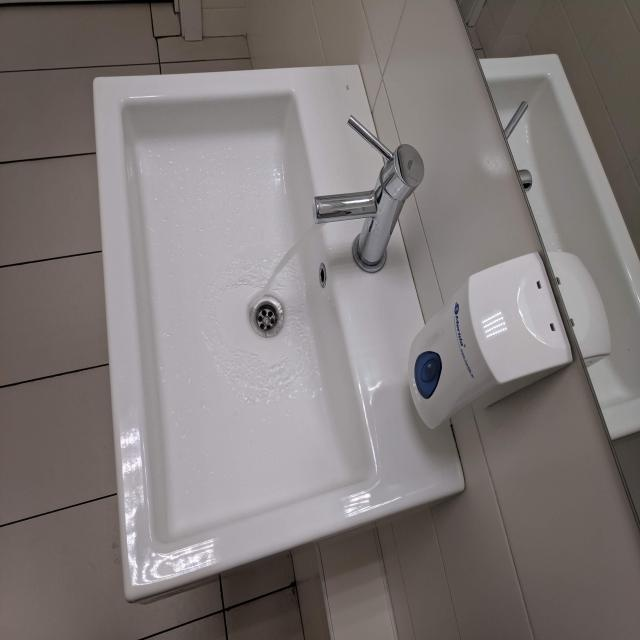
\includegraphics[width=0.475\linewidth]{figures/yolov5-prediction-2.jpg}%
        \hfill
        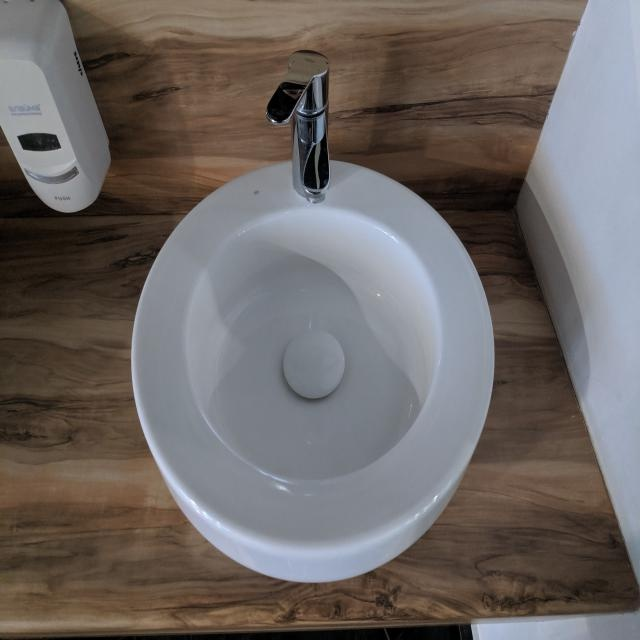
\includegraphics[width=0.475\linewidth]{figures/yolov5-prediction-3.jpg}%
        \hfill
        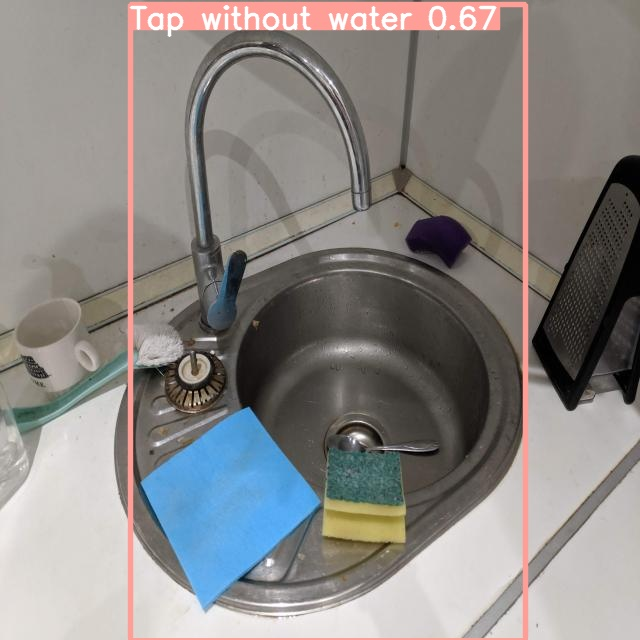
\includegraphics[width=0.475\linewidth]{figures/yolov5-prediction-4.jpg}
    \end{subfigure}
    \caption{Predictions of YOLOv5 Nano on the test portion of the dataset}
\end{figure}

\subsection{Performance of Mask R-CNN}

Mask R-CNN had a more difficult task than the previous two models – it also had to predict the mask of a tap. The calculated mAP is 0.7, but the predictions are not very accurate in this case either. For example, in \textbf{Fig. 8}, the model predicted both running water and no water with relatively high confidence, the ground truth receiving even less confidence than the other class. The mask was detected, although roughly, around the tap.

\begin{figure}[htb]
    \centering
    \begin{subfigure}[b]{\textwidth}
        \centering
        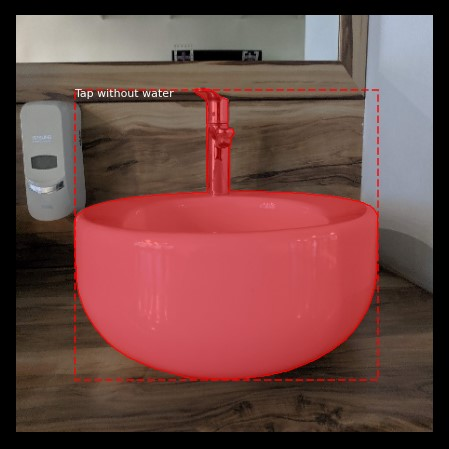
\includegraphics[width=0.475\linewidth]{figures/mask-rcnn-truth.jpg}%
        \hfill
        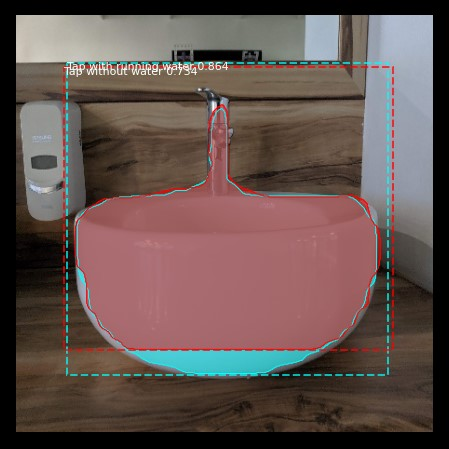
\includegraphics[width=0.475\linewidth]{figures/mask-rcnn-prediction.jpg}
    \end{subfigure}
    \caption{Ground truth (left) and the prediction of Mask R-CNN (right) on an image from the test set}
\end{figure}

\section{Conclusion}

As anticipated, the task of detecting running water was challenging for the models. However, the implications of this experiment must be considered – small dataset, smallest versions of models, lack of hyperparameter finetuning. YOLOv4 seems to have produced the best result in this task, which is supported by its mAP metric, even though it might not exactly reflect the truth of the test dataset.

The source code of this experiment is available on GitHub\footnote{\href{https://github.com/illright/cvdl-save-water-iu-f21}{\texttt{illright/cvdl-save-water-iu-f21} on GitHub}}, with the dataset and the notebooks with outputs in the \emph{Releases} section.

\end{document}
